%! Author = trevo
%! Date = 2/22/2025

% Preamble
\documentclass[12pt]{report}
\usepackage{amsmath,geometry,setspace, enumerate,pdfpages,mathrsfs,hyperref,csquotes,graphicx,amsfonts,pdfpages}
\usepackage[british]{babel}
\usepackage[round]{natbib}
\bibliographystyle{plainnat}
\doublespacing
\setlength\parindent{24pt}
\setcounter{tocdepth}{3}



\begin{document}

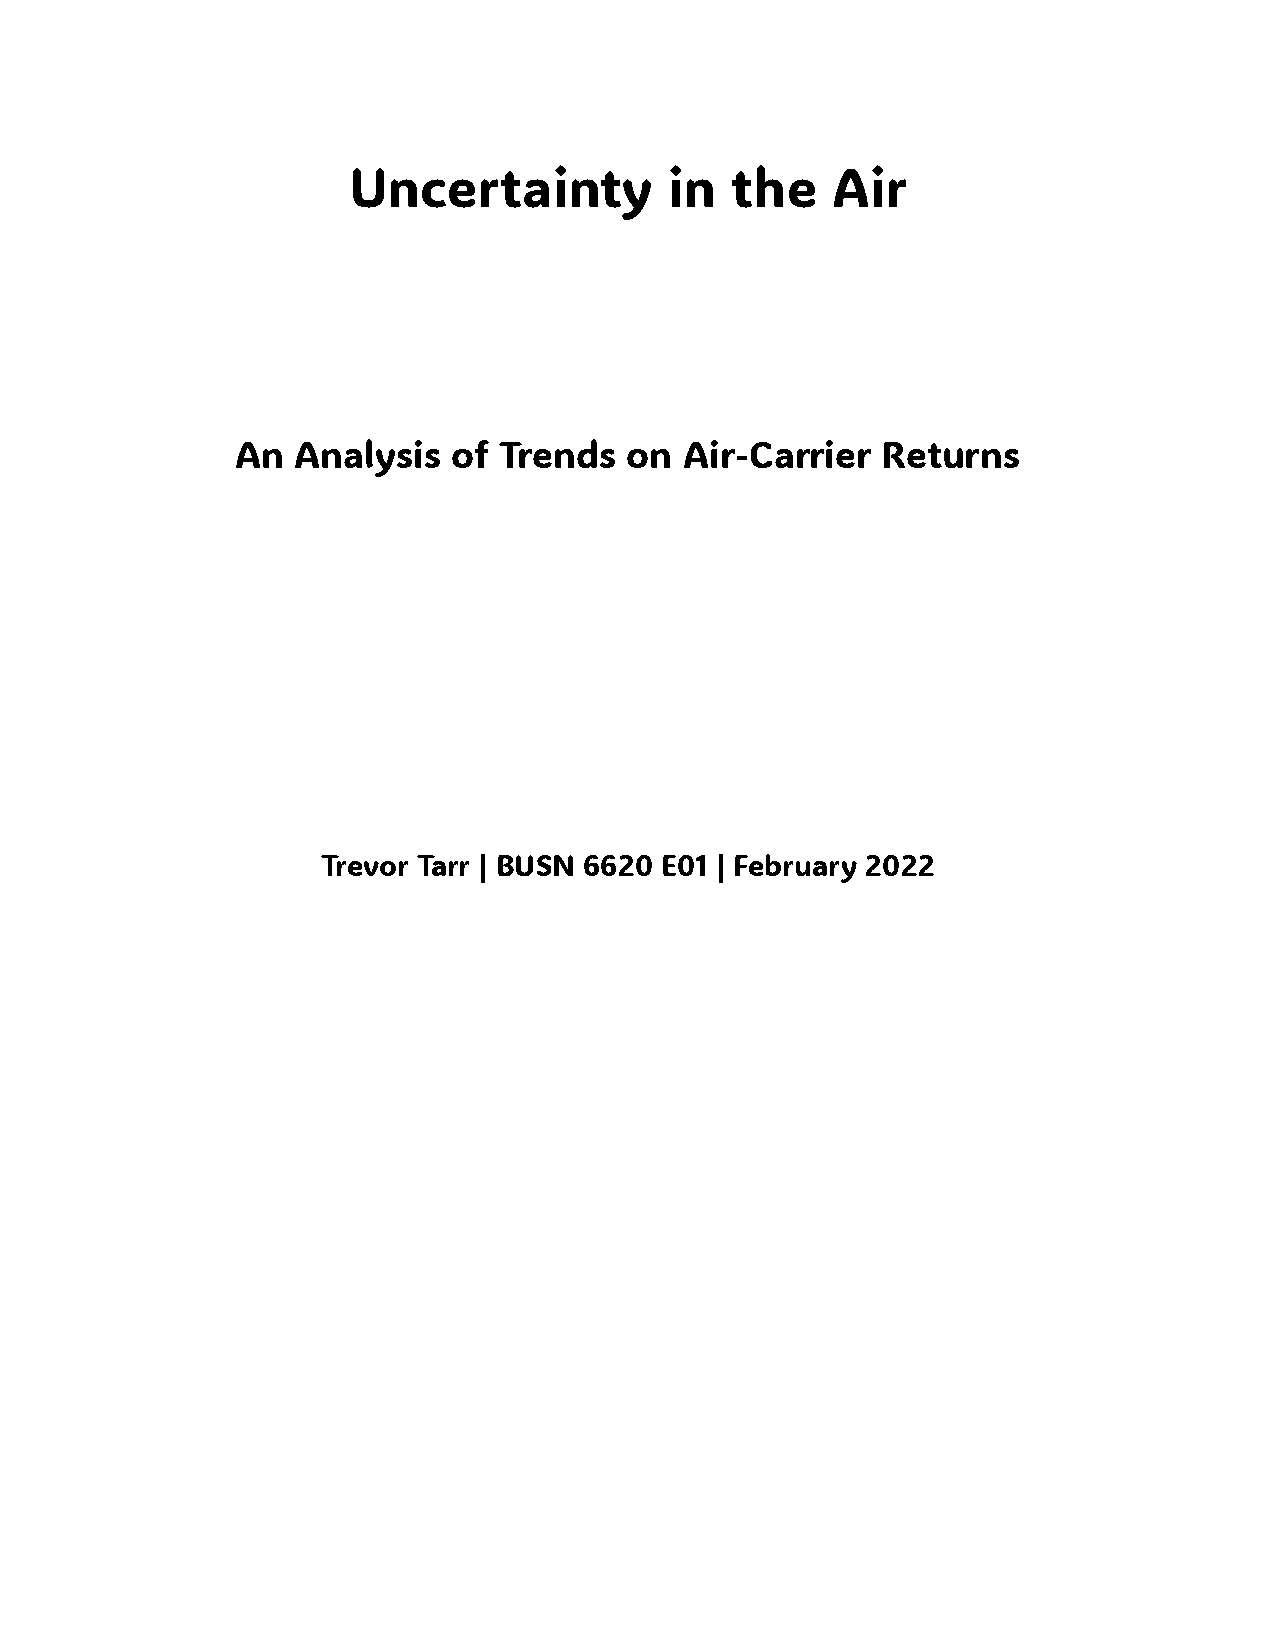
\includepdf{F2DTP}
    \newpage
\pagenumbering{gobble}
    \newpage
    \pagenumbering{roman}


\newpage
\tableofcontents
\newpage

\pagenumbering{arabic}
\chapter*{Abstract, Hypothesis, Motivation}
\addcontentsline{toc}{chapter}{Abstract, Hypothesis, Motivation}
\section*{\underline{Abstract}}
\addcontentsline{toc}{section}{Abstract}

\section*{\underline{Hypothesis}}
\addcontentsline{toc}{section}{Hypothesis}

\section*{\underline{Motivation}}
\addcontentsline{toc}{section}{Motivation}

\nocite{*}

\newpage
\chapter*{Methodology}
\addcontentsline{toc}{chapter}{Methodology}
\section*{\underline{Variables}}
\addcontentsline{toc}{section}{Variables}
\begin{enumerate}
 \item[\underline{Independent}]: Trend Data (Google Trend Data).
   \addcontentsline{toc}{subsection}{Independent}
    These trend topics are to encapsulate various issues, risks, and interests theorized to impact the airline market.
        \begin{enumerate}
            \item[Travel Restriction]: This topic was chosen to highlight the news and trends on when travel is disrupted due to political or physical barriers to travel.
            This includes during pandemics, political instability, economic instability, infrastructure changes, or other factor disrupting travel.
            \item[Boeing Plane]: Boeing is one of the main manufacturers of commercial aircraft.
            This topic was chosen to highlight news on a supply line of an air-carrier.
            \item[Airbus Plane]: Airbus is the main competitor of Boeing in regard to the commercial aircraft manufacturing market.
            This topic was chosen to highlight and compare to Boeing Plane Trends.
            \item[Pilot Strike]: Pilots are the main employment positions for an air-carrier organization.
            This topic was chosen to highlight disruptions in the labour market category for air-carrier organizations.
            \item[Terrorism]: Terrorist acts create a sense of fear in customers to travel.
            This topic was chosen to highlight the travel demand with the news of fear and the threat of physical danger whether at home or abroad.
        \end{enumerate}
{\tiny Note: Singular forms were chosen over plural to account for seperated events involving planes, strikes, and restrictions.}


  \addcontentsline{toc}{subsection}{Dependent}
    \item[\underline{Dependent}]: Airline Closing Monthly Stock Prices.
    The airlines chosen are a sample from both Legacy and Low-Cost carriers as to observe trend data on both sectors within the industry.
    \begin{enumerate}
        \item[Legacy]: Airlines flying prior to airline deregulation in the 1970s and typically seen as luxury brands.
            \begin{enumerate}
                \item[1.]Delta Air Lines, Inc. (DAL)
                \item[2.]United Airlines Holdings, Inc. (UAL)
            \end{enumerate}
        \item[Low-Cost]: Airlines who focus on providing the basic flight packages rather than luxury travel.This lowers teh costs of flying for customers but at the cut of luxuries that may include: full meal options, broad entertainment options, seat classes, etc. .
            \begin{enumerate}
                \item[3.]Southwest Airlines Co. (LUV)
                \item[4.]Allegiant Travel Company (ALGT)
            \end{enumerate}
    \end{enumerate}


\end{enumerate}

\section*{\underline{Data Collection}}
\addcontentsline{toc}{section}{Data Collection}

Data collection for Dependent Variables was gathered from Historical Data from Yahoo Finance using tickers: UAL, DAL, LUV, ALGT. This data was then transferred to a Microsoft Excel notebook.
\\ \\
Data collection for Independent variables were gathered from worldwide monthly Google Trend data values over the maximum amount stored by Google Trends (2004 onwards).
This data was downloaded as a .csv file and opened and used in a separate Microsoft Excel sheet in the same notebook as the Dependent variable data.


\section*{\underline{Analysis Methodology}}
\addcontentsline{toc}{section}{Analysis Methodology}




\newpage
\chapter*{Results and Interpertations}
\addcontentsline{toc}{chapter}{Results and Interpertations}

\section*{\underline{United}}
\addcontentsline{toc}{section}{United}
\subsection*{Results:}
\begin{enumerate}
    \item[\underline{Travel Restriction:}]
        \begin{enumerate}
            \item[$R^2$]:
            \item[Coefficient Value]:
            \item[Coefficient t-stat]:
        \end{enumerate}
    \item[\underline{Boeing Plane:}]
        \begin{enumerate}
            \item[$R^2$]:
            \item[Coefficient Value]:
            \item[Coefficient t-stat]:
        \end{enumerate}
    \item[\underline{Airbus Plane:}]
        \begin{enumerate}
            \item[$R^2$]:
            \item[Coefficient Value]:
            \item[Coefficient t-stat]:
        \end{enumerate}
    \item[\underline{Pilot Strike:}]
        \begin{enumerate}
            \item[$R^2$]:
            \item[Coefficient Value]:
            \item[Coefficient t-stat]:
        \end{enumerate}
    \item[\underline{Terrorism:}]
        \begin{enumerate}
            \item[$R^2$]:
            \item[Coefficient Value]:
            \item[Coefficient t-stat]:
        \end{enumerate}
    \item[\underline{All:}]
        \begin{enumerate}
            \item[$R^2$]:
            \item[Coefficient Value]:
            \item[Coefficient t-stat]:
        \end{enumerate}
\end{enumerate}
\subsection*{Interpretation:}

\newpage
\section*{\underline{Delta}}
\addcontentsline{toc}{section}{Delta}
\subsection*{Results:}
\begin{enumerate}
    \item[\underline{Travel Restriction:}]
        \begin{enumerate}
            \item[$R^2$]:
            \item[Coefficient Value]:
            \item[Coefficient t-stat]:
        \end{enumerate}
    \item[\underline{Boeing Plane:}]
        \begin{enumerate}
            \item[$R^2$]:
            \item[Coefficient Value]:
            \item[Coefficient t-stat]:
        \end{enumerate}
    \item[\underline{Airbus Plane:}]
        \begin{enumerate}
            \item[$R^2$]:
            \item[Coefficient Value]:
            \item[Coefficient t-stat]:
        \end{enumerate}
    \item[\underline{Pilot Strike:}]
        \begin{enumerate}
            \item[$R^2$]:
            \item[Coefficient Value]:
            \item[Coefficient t-stat]:
        \end{enumerate}
    \item[\underline{Terrorism:}]
        \begin{enumerate}
            \item[$R^2$]:
            \item[Coefficient Value]:
            \item[Coefficient t-stat]:
        \end{enumerate}
    \item[\underline{All:}]
        \begin{enumerate}
            \item[$R^2$]:
            \item[Coefficient Value]:
            \item[Coefficient t-stat]:
        \end{enumerate}
\end{enumerate}
\subsection*{Interpretation:}

\newpage
\section*{\underline{Southwest}}
\addcontentsline{toc}{section}{Southwest}
\subsection*{Results:}
\begin{enumerate}
    \item[\underline{Travel Restriction:}]
        \begin{enumerate}
            \item[$R^2$]:
            \item[Coefficient Value]:
            \item[Coefficient t-stat]:
        \end{enumerate}
    \item[\underline{Boeing Plane:}]
        \begin{enumerate}
            \item[$R^2$]:
            \item[Coefficient Value]:
            \item[Coefficient t-stat]:
        \end{enumerate}
    \item[\underline{Airbus Plane:}]
        \begin{enumerate}
            \item[$R^2$]:
            \item[Coefficient Value]:
            \item[Coefficient t-stat]:
        \end{enumerate}
    \item[\underline{Pilot Strike:}]
        \begin{enumerate}
            \item[$R^2$]:
            \item[Coefficient Value]:
            \item[Coefficient t-stat]:
        \end{enumerate}
    \item[\underline{Terrorism:}]
        \begin{enumerate}
            \item[$R^2$]:
            \item[Coefficient Value]:
            \item[Coefficient t-stat]:
        \end{enumerate}
    \item[\underline{All:}]
        \begin{enumerate}
            \item[$R^2$]:
            \item[Coefficient Value]:
            \item[Coefficient t-stat]:
        \end{enumerate}
\end{enumerate}
\subsection*{Interpretation:}

\newpage
\section*{\underline{Allegiant}}
\addcontentsline{toc}{section}{Allegiant}
\subsection*{Results:}
\begin{enumerate}
    \item[\underline{Travel Restriction:}]
        \begin{enumerate}
            \item[$R^2$]:
            \item[Coefficient Value]:
            \item[Coefficient t-stat]:
        \end{enumerate}
    \item[\underline{Boeing Plane:}]
        \begin{enumerate}
            \item[$R^2$]:
            \item[Coefficient Value]:
            \item[Coefficient t-stat]:
        \end{enumerate}
    \item[\underline{Airbus Plane:}]
        \begin{enumerate}
            \item[$R^2$]:
            \item[Coefficient Value]:
            \item[Coefficient t-stat]:
        \end{enumerate}
    \item[\underline{Pilot Strike:}]
        \begin{enumerate}
            \item[$R^2$]:
            \item[Coefficient Value]:
            \item[Coefficient t-stat]:
        \end{enumerate}
    \item[\underline{Terrorism:}]\\
        \begin{enumerate}
            \item[$R^2$]:
            \item[Coefficient Value]:
            \item[Coefficient t-stat]:
        \end{enumerate}
    \item[\underline{All:}]
        \begin{enumerate}
            \item[$R^2$]:
            \item[Coefficient Value]:
            \item[Coefficient t-stat]:
        \end{enumerate}
\end{enumerate}
\subsection*{Interpretation:}

\newpage


\chapter*{Conclusion, Recommendations, \& Bibliography}
\addcontentsline{toc}{chapter}{Conclusion, Recommendations \& Bibliography}
\section*{Conclusion}
\addcontentsline{toc}{section}{Conclusion}

\section*{Recommendations}
\addcontentsline{toc}{section}{Recommendations}
\newpage






    \bibliography{resources}
    \addcontentsline{toc}{section}{Bibliography}
\end{document}
